% $HeadURL$

\subsection{Glyph: \glyph{Nucleic acid feature}}
\label{sec:genetic}

The \emph{Nucleic acid feature} construct in SBGN is meant to represent a fragment of a macromolecule carrying genetic information.  A common use for this construct is to represent a gene or transcript.  The label of this EPN and its \emph{units of information} are often important for making the purpose clear to the reader of a map.

\begin{glyphDescription}

\glyphSboTerm SBO:0000354 !  informational molecule segment

\glyphContainer A \glyph{nucleic acid feature} is represented by a rectangular container whose bottom half has rounded corners, as shown in \fig{genetic}. This design reminds that we are fundamentally dealing with a unit of information, but this information is carried by a macromolecule.

\glyphLabel The identity of a particular \glyph{Nucleic acid feature} is established by a label placed in an unordered box containing a string of characters.  The characters may be distributed on several lines to improve readability, although this is not mandatory.  The label box must be attached to the center of the container.  The label may spill outside of the container.

\glyphAux A \glyph{nucleic acid feature} can carry state variables (\sect{stateVariable}) that add information about its precise state.  The state of a \glyph{nucleic acid feature} is therefore defined as the vector of all its state variables. 

A \glyph{nucleic acid feature} can also carry one or several \glyph{units of information} (\sect{unitInfo}).  These can characterize a \glyph{nucleic acid feature}'s domain, such as a binding site, or an exon.  Particular \glyph{units of information} carry the material type (\sect{material-types-cv}) and the conceptual type (\sect{conceptual-types-cv}) of the \glyph{nucleic acid feature}. 

A \glyph{nucleic acid feature} may also carry a \glyph{clone marker}
(\sect{cloneMarker}).

\end{glyphDescription}


\begin{figure}[H]
  \centering
  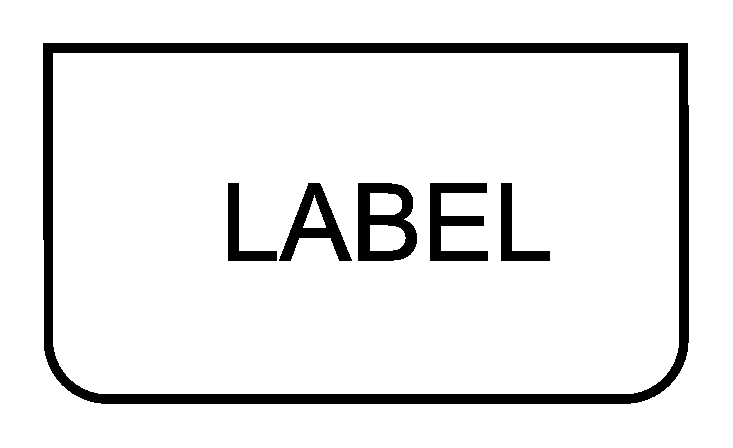
\includegraphics[width = 1.25in]{images/genetic-plain} \hspace*{2em}
  \raisebox{0.04in}{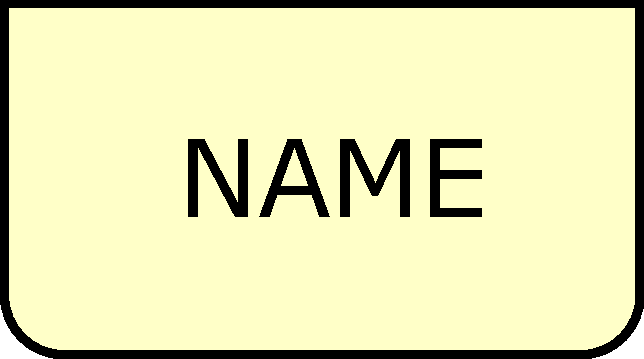
\includegraphics[width = 1.25in]{images/genetic}}
  \caption{The \PD glyph for \glyph{nucleic acid feature}, shown plain and
    unadorned on the left and with an additional state variable and a
    unit of information on the right.} 
  \label{fig:genetic}
\end{figure}

% The following is for [X]Emacs users.  Please leave in place.
% Local Variables:
% TeX-master: "../sbgn_PD-level1"
% End:
